\chapter{Manual juego en 3D}

\section{Estructura de las escenas}

La estructura del videojuego es la siguiente: 

\begin{figure}[H]
	\centering
	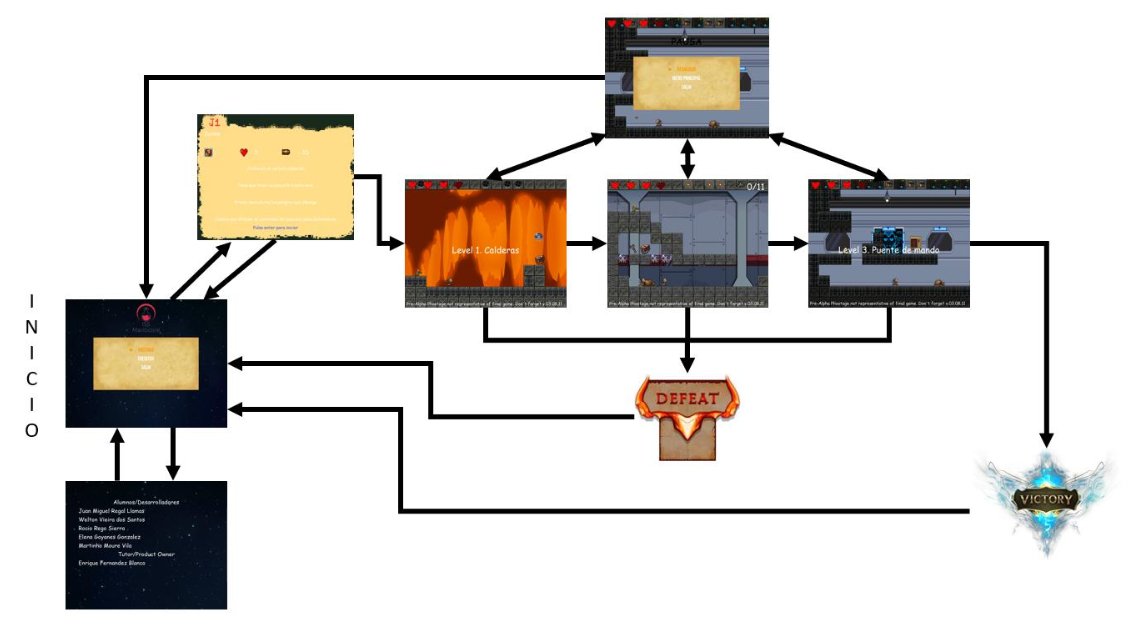
\includegraphics[scale=0.50]{imagenes/Estructura_escena.png}
	\caption{\label{fig:Estructura_escena}Estructura de las escenas del video juego}
\end{figure}

\section{Controles}

Las teclas WASD y las flechas del teclado permiten que el jugador se mueva por el escenario en las direcciones de las flechas. Para manejar la cámara, es decir, lo que ve el personaje se utiliza el ratón para ese cometido. Figura \ref{fig:flechasTeclado}.

\begin{figure}[H]
	\centering
	\includegraphics[scale=0.40]{imagenes/teclasWASD.png}
	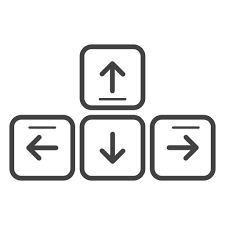
\includegraphics[scale=0.50]{imagenes/flechas_teclado.png}
	\caption{\label{fig:flechasTeclado}Teclas de movimiento del personaje}
\end{figure}

El ratón permite que el jugador apunte y dispare los proyectiles a sus enemigos con click izquierdo.

\begin{figure}[H]
	\centering
	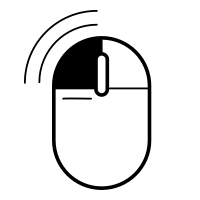
\includegraphics[scale=0.50]{imagenes/raton.png}
	\caption{\label{fig:raton}Raton y click izquierdo}
\end{figure}

La tecla escape permite al jugador acceder al menú de pausa
\begin{figure}[H]
	\centering
	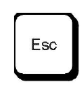
\includegraphics[scale=0.50]{imagenes/escape.png}
	\caption{\label{fig:escape}Tecla escape}
\end{figure}

\section{Ejecución del juego}
Para ejecutar el juego  basta el ejecutar el archivo ejecutable del juego.

\section{Navegación del Menu Principal}
Al iniciarse el juego aparece el menú de inicio con las siguientes opciones: 

\begin{figure}[H]
	\centering
	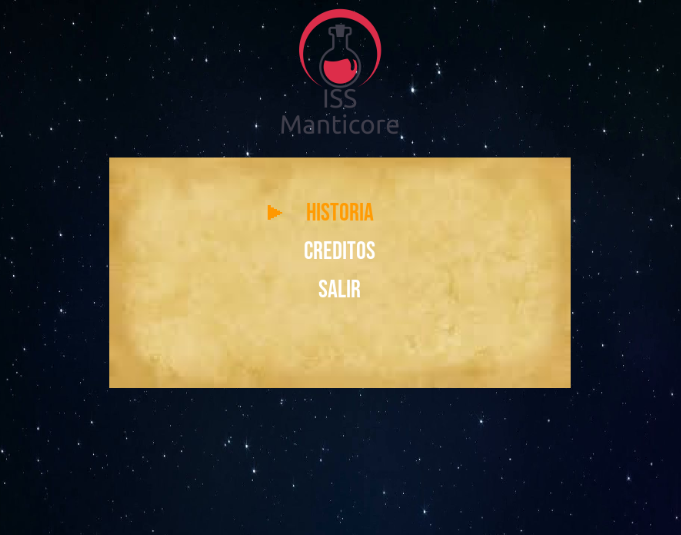
\includegraphics[scale=0.50]{imagenes/EjemploMenuPrincipal.png}
	\caption{\label{fig:EjemploMenuPrincipal}Ejemplo del menu principal}
\end{figure}

Para desplazarse entre las distintas opciones se utilizan las flechas del teclado y para seleccionarla se pulsa Enter.  

A continuación, se detallan cada una de ellas: 
\begin{itemize}
	\item \textbf{Historia:} muestra la leyenda del juego, con la configuración inicial en la que aparece la imagen del personaje, la cantidad de vida con la que comienza el jugador y la cantidad de munición (para como ya se mencionó implementar en el juego un sistema de munción y armas complejo en el futuro) 
	\item \textbf{Créditos:} muestra la lista de nombres de los desarrolladores y del product owner.  
	\item \textbf{Salir:} cierra la ventana del juego. 
\end{itemize}



Tanto desde la pantalla de la leyenda como desde los créditos se puede retroceder al menú pulsando la tecla Esc. 


Cuando da comienzo la historia van apareciendo los diferentes niveles que el jugador debe superar, si este llega al final aparecerá un indicativo demostrando que ha finalizado el juego. Si por el contrario el jugador pierde todas sus vidas por el camino aparecerá otro indicativo manifestando la derrota. Tras terminar el juego, tanto con éxito como si no, es necesario pulsar la tecla Esc para volver al menú principal.    